\section{Experiments}\label{sec:expts}


\subsection{Methods Compared}

We refer to the multi-user variant of our model as \emph{crowd-GPPL}.
As baselines, we use GPPL to learn a single preference function from all users' preference labels, (\emph{GPPL-pooled}), and a Gaussian process over the joint feature space of users and items 
(\emph{GPPL-joint}), as proposed by \citet{guo2010gaussian}.
For datasets up to 100 users (simulated data, subsamples of the real datasets), 
we also test separate GPPL instances per user with no collaborative
learning (\emph{GPPL-per-user}), but this could not be applied to the real datasets as the 
computation costs were too high.
To test the benefit of using GPs to model item and user features,
we also test two further baselines: 
\emph{crowd-GPPL$\mathbf{\setminus \bs u}$}, which ignores the user features,
and \emph{crowd-BMF}, which ignores both user and item features and so does not use GPs at all. 
For both of these methods, the user covariance matrix, $\bs K_w$, in the crowd-GPPL model is replaced by the identity matrix, and for \emph{crowd-BMF}, the item covariance matrices, $\bs K_v$ and $\bs K_t$ are also replaced by the identity matrix.

% Ranking-SVM baseline -- only easy to compare in the single user case. My GPPL paper perhaps needs
% this adding in any follow up works.

% Houlsby tests: with/without user features (without is better with few users). + a hierarchical 
% model, BI (multi task preference learning, Birlitiu et al), and the GPPL-joint model. None of 
% these are done at scale, which we can do with our inference method --> *this is a new claim i.e. 
% new empirical results*. They also test a per-user model.

\subsection{Datasets}

\subsection{Simulated Noisy Data}\label{sec:exp_synth}

Dataset:

Hypothesis: 

\begin{figure}
\includegraphics[scale=1]{../../results/synth_sandbox/single_user/tau_test}
\includegraphics[scale=1]{../../results/synth_sandbox/multi_user_consensus/tau_test}
\includegraphics[scale=1]{../../results/synth_sandbox/multi_user_personal/tau_test}
\caption{Recovering latent preference functions with increasing levels of noise
in different scenarios: 
(a) single user; 
(b) ground truth function from crowdsourced labels; 
(c) latent components from a crowd of users.
}
\end{figure}

\begin{figure}
\includegraphics[scale=1]{../../results/synth_sandbox/multiuser_factor_correlations_s/noise_r}
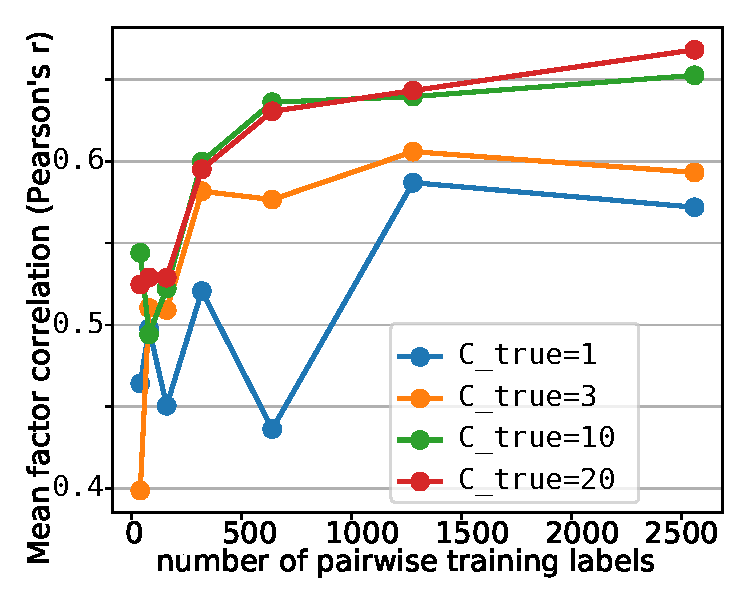
\includegraphics[scale=1]{../../results/synth_sandbox/multiuser_factor_correlations_P/num_pairs_r}
\caption{Correlations between the inferred and ground truth latent factors with varying values of
(a) noise variance, s; 
(b) number of pairwise labels in training data. 
}
\end{figure}

\subsection{Sushi Preferences}\label{sec:exp_small}

Dataset: Sushi
% Houlsby results: for comparison against a different inference technique on small data, include
% the test error results from their paper.
% Guo results: not directly comparable. We will rerun a similar approach but with our inference method.
% Khan results: for a different model that separates the latent features from the item/user features.
% Abbasnejad results (community-based preference learning): sushi data with 10 items; 60/40 train/test split of each user's preference pairs. This means the result is based on 27 pairs training.
% don't worry about this though, it doesn't seem to work very well in their results.

Hypothesis: 
% Number of users affects value of including user features.
% Plot results on increasing dataset size.

% [10] T. Kamishima. Nantonac collaborative filtering:
% Recommendation based on order responses. In
% ACM SIGKDD 9th Int. Conf. Knowledge Discov-
% ery and Data Mining, 2003.

Setup:

Run 25 repeats of random train/test splits with:
% Exclude these two as we focus on bigger datasets in this paper. Cutting these creates the space 
% for including three metrics.
% Downside: cannot test whether increasing no. users imroves performance through better collaborative learning. 
% 
% 100 (a la Houlsby 20 pairs per user), 
% 200 (a la Khan, 3 training, 1 test, P=600, P_test=200), 
% For small datasets, we may want to test on the argumentation data so we can assess the crowd
% consensus results with small data. That dataset is more interesting here because lots of items,
% small data is a new scenario.
[a] 1000 (a la Houlsby 15 training, 5 test pairs per user, $P=15000,P_{test}=5000$), Sushi-A (10 items), 
and [b] 5000 users (a la Khan, 10 training, 1 test pairs per user, $P=50000, P_{test}=5000$), Sushi-B (100 items).
Evaluate on parwise labelling error, pairwise label logloss, spearman rank correlation,
and runtime.
% could use normalized mean loss from guo, but not sure where the utilities come from -- ranking?

% 25 random train/test splits on all 5000 users with varying no. (1, 5, 10, 20, 40) pairs per user.

% Can put in the Houlsby (100/1000 users, 20 pairs each, labelling error) and Khan (200 users, 3 pairs each, logloss) results.
% Khan also provide code, so could be rerun to get classification error.

% Also consider whether we can show more results in a table format?

In all cases, we use the no. pairs per user and no. users to select the subset of data used for training, then test on the remainder.

\begin{table}
\begin{tabularx}{\textwidth}{| l | c | c | c | c |}
\\ \hline
%\input{../../results/sushi_10_4/results.tex}\\
%\input{../../results/sushi_10_opt_4/results.tex}\\
\\ \hline
\end{tabularx}
\caption{Performance on Sushi-A dataset with 10 items, 1000 users, 15 pairwise labels per user for training.}
\end{table}

\begin{table}
\begin{tabularx}{\textwidth}{| l | c | c | c | c |}
\\ \hline
%\input{../../results/sushi_100_4/results.tex} \\ 
%\input{../../results/sushi_100_opt_4/results.tex} \\
\\ \hline
\end{tabularx}
\caption{Performance on Sushi-B dataset with 100 items, 5000 users, 10 pairwise labels per user for training.}
\end{table}

\begin{figure}
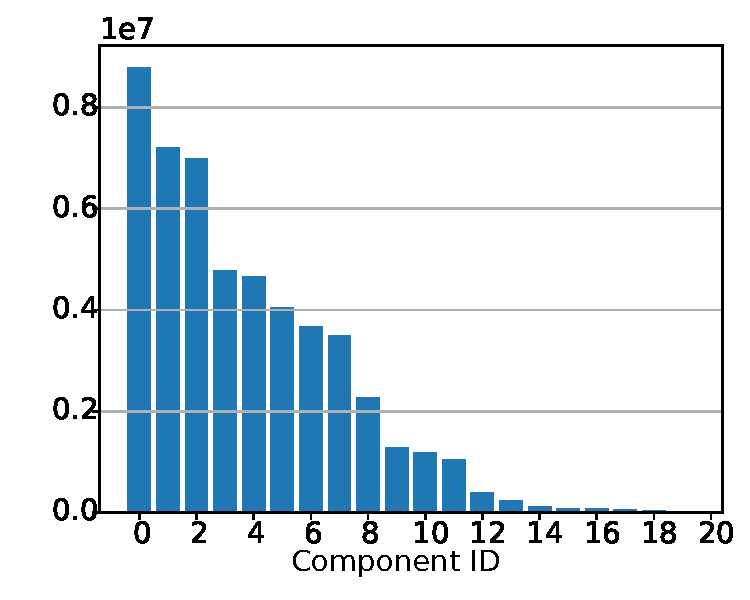
\includegraphics[scale=1]{../../results/sushi_factor_scales}
\caption{
Distribution of latent factor variances, $s_c$, for crowd-GPPL on the Sushi-A and Sushi-B datasets, averaged over all $25$ runs.
}
\end{figure}

\section{Scalability Experiments}\label{sec:exp_scale}

Dataset:

Hypothesis: 

List of experiments to include -- need new plots for the crowd model:
\begin{enumerate}
\item Performance, computation time vs. no. inducing points
\item Computation time vs. dataset size, no. features
%\item not done: memory vs no. inducing points, update size
%\item not done: Performance, computation time, vs update size
%%\item not done: performance, computation time vs different initialisation methods for the inducing points; include different initialisations of K-means
\end{enumerate}

\begin{figure}
\subfloat[Varying number of items in training set. GloVe features.]{
    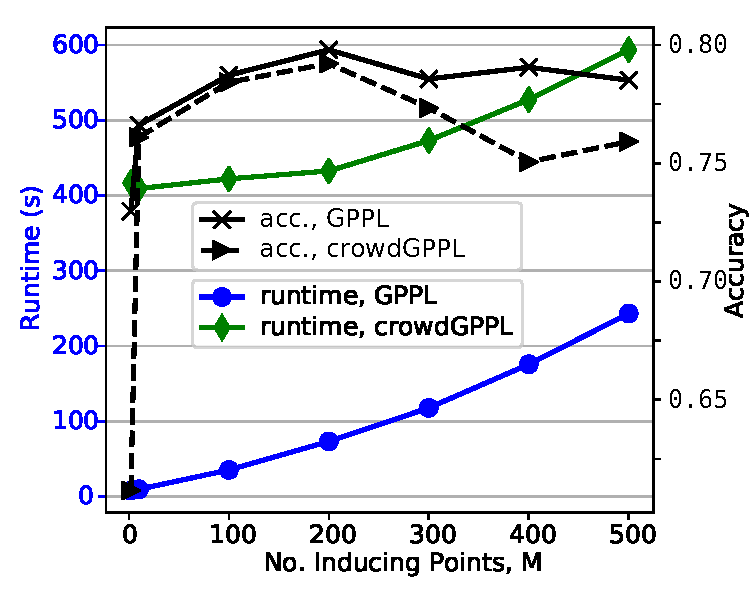
\includegraphics[scale=1]{../../results/scalability/num_inducing_32310_features}
}
\subfloat[Varying no. ling+GloVe features. $M=500$]{
    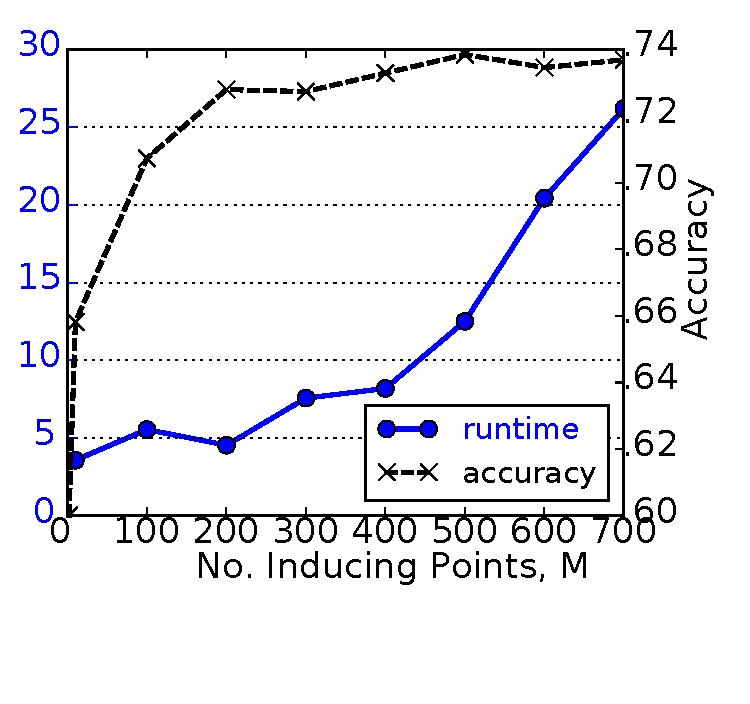
\includegraphics[scale=1]{../../results/scalability/num_inducing_300_features}
}
\caption{
    Runtimes for training+prediction on UKPConvArgCrowdSample with varying subsample size. Means over 32 runs. 
    Note the logarithmic x-axis for (b).
}
\end{figure}
\begin{figure}
\subfloat[33210 ling+GloVe features]{
    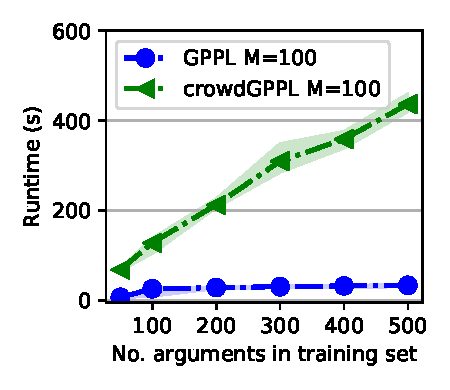
\includegraphics[scale=1]{../../results/scalability/num_arguments}
}
\subfloat[300 GloVe features]{
    \includegraphics[scale=1]{../../results/scalability/num_features}
}
\caption{
Effect of varying $M$ on accuracy and runtime (training+prediction) for GPPL and crowd-GPPL on UKPConvArgCrowdSample. Means over 32 runs.
}
\end{figure}

\section{Argument Convincingness}\label{sec:exp_nlp}

We compare performance of several methods on the Dataset used in Section \ref{sec:exp_scale}.

Methods: 

Hypothesis: 


\begin{table}
\begin{tabularx}{\columnwidth}{ | l | X | X | X | X | X | X |}
\hline
 & \multicolumn{3}{|X|}{Consensus}&\multicolumn{3}{| X |}{Personal} \\ \hline
 Method & Acc & CEE & Kend. & Acc & CEE & Kend. \\ \hline
 SVM & .70 & .58 & .31 & & &  \\
 Bi-LSTM & .73 &  .55 & .21 & & & \\
 GPPL medi. & \textbf{.77} & \textbf{.50} &  \textbf{.40} & & &  \\
 GPPL opt. & & & & & &  \\
 Crowd-GPPL medi. & & & & & & \\
 Crowd-GPPL opt. & & & & & & \\
 PL+ SVR & .75 & .55 & \textbf{.40} & & & \\
 GPC & .73 & .53 & - & & & - \\
 \\\hline
\end{tabularx}
\caption{Performance comparison on UKPConvArgCrowdSample using ling+GloVe features. \emph{Acc} and \emph{CEE} show classification accuracy and cross entropy error (or log-loss) for pairwise predictions, 
while \emph{Kend.} shows Kendall's tau for the predicted preference function.}
\label{tab:convarg}
\end{table}

\begin{figure}
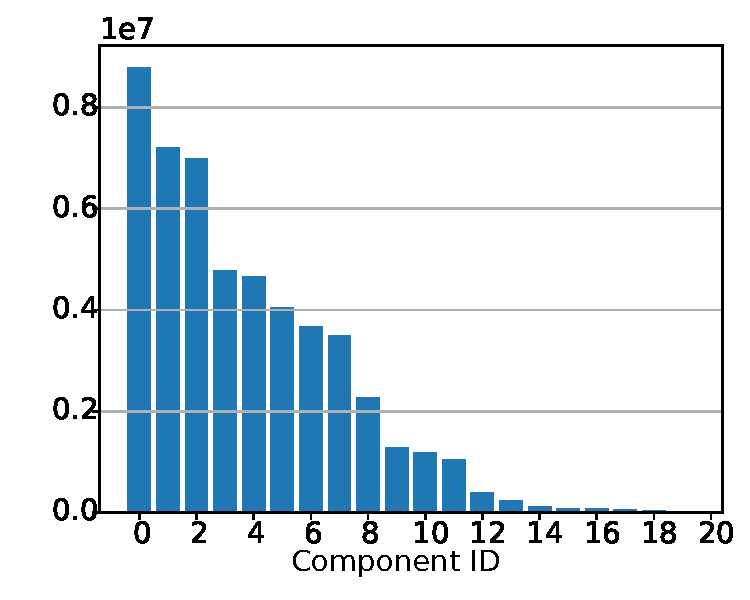
\includegraphics[scale=1]{../../results/sushi_factor_scales}
\caption{
Distribution of latent factor variances, $s_c$, for crowd-GPPL on UKPConvArgCrowdSample, averaged over all $32$ runs.
}
\end{figure}